%%%%%%%%%%%%%%%%%%%%%%%%%%%%%%%%%%%%%%%%%
% Beamer Presentation
% LaTeX Template
% Version 1.0 (10/11/12)
%
% This template has been downloaded from:
% http://www.LaTeXTemplates.com
%
% License:
% CC BY-NC-SA 3.0 (http://creativecommons.org/licenses/by-nc-sa/3.0/)
%
%%%%%%%%%%%%%%%%%%%%%%%%%%%%%%%%%%%%%%%%%

%----------------------------------------------------------------------------------------
%	PACKAGES AND THEMES
%----------------------------------------------------------------------------------------

\documentclass{beamer}

\mode<presentation> {

% The Beamer class comes with a number of default slide themes
% which change the colors and layouts of slides. Below this is a list
% of all the themes, uncomment each in turn to see what they look like.

%\usetheme{default}
%\usetheme{AnnArbor}
%\usetheme{Antibes}
%\usetheme{Bergen}
%\usetheme{Berkeley}
%\usetheme{Berlin}
%\usetheme{Boadilla}
%\usetheme{CambridgeUS}
%\usetheme{Copenhagen}
%\usetheme{Darmstadt}
\usetheme{Dresden}
%\usetheme{Frankfurt}
%\usetheme{Goettingen}
%\usetheme{Hannover}
%\usetheme{Ilmenau}
%\usetheme{JuanLesPins}
%\usetheme{Luebeck}
%\usetheme{Madrid}
%\usetheme{Malmoe}
%\usetheme{Marburg}
%\usetheme{Montpellier}
%\usetheme{PaloAlto}
%\usetheme{Pittsburgh}
%\usetheme{Rochester}
%\usetheme{Singapore}
%\usetheme{Szeged}
%\usetheme{Warsaw}

% As well as themes, the Beamer class has a number of color themes
% for any slide theme. Uncomment each of these in turn to see how it
% changes the colors of your current slide theme.

%\usecolortheme{albatross}
%\usecolortheme{beaver}
%\usecolortheme{beetle}
%\usecolortheme{crane}
%\usecolortheme{dolphin}
%\usecolortheme{dove}
%\usecolortheme{fly}
%\usecolortheme{lily}
%\usecolortheme{orchid}
%\usecolortheme{rose}
%\usecolortheme{seagull}
%\usecolortheme{seahorse}
%\usecolortheme{whale}
%\usecolortheme{wolverine}

%\setbeamertemplate{footline} % To remove the footer line in all slides uncomment this line
%\setbeamertemplate{footline}[page number] % To replace the footer line in all slides with a simple slide count uncomment this line

%\setbeamertemplate{navigation symbols}{} % To remove the navigation symbols from the bottom of all slides uncomment this line
}

\usepackage{graphicx} % Allows including images
\usepackage{booktabs} % Allows the use of \toprule, \midrule and \bottomrule in 
%tables
\usepackage{listings}

%----------------------------------------------------------------------------------------
%	TITLE PAGE
%----------------------------------------------------------------------------------------

\title[Lecture 1]{Advanced R Programming - Lecture 1} % The short title 
%appears at the bottom of every slide, the full title is only on the title page

\author{Leif Jonsson} % Your name
\institute[STIMA LiU] % Your institution as it will appear on the bottom of 
%every 
%slide, may be shorthand to save space
{
Link\"{o}ping University \\ % Your institution for the title page
\medskip
\textit{leif.jonsson@ericsson.com\\leif.r.jonsson@liu.se} % Your email address
}
\date{\today} % Date, can be changed to a custom date

\begin{document}

\begin{frame}
\titlepage % Print the title page as the first slide
\end{frame}

\begin{frame}
\frametitle{Today} % Table of contents slide, comment this block out to remove 
%it
\tableofcontents % Throughout your presentation, if you choose to use \section{} and \subsection{} commands, these will automatically be printed on this slide as an overview of your presentation
\end{frame}

%----------------------------------------------------------------------------------------
%	PRESENTATION SLIDES
%----------------------------------------------------------------------------------------

%------------------------------------------------
\section{About the course} % Sections can be created in order to organize your 
%presentation into discrete blocks, all sections and subsections are 
%automatically printed in the table of contents as an overview of the talk
%------------------------------------------------

\subsection{Aim of the course} % A subsection can be created just before a set 
%of slides with a common theme to further break down your presentation into 
%chunks
%------------------------------------------------

\begin{frame}
\frametitle{Learn to}
\begin{itemize}
\item Write R programs and packages
\item Write performant code
\item Learn basic software engineering practices
\end{itemize}
\end{frame}

\begin{frame}
	\frametitle{But most important...}
\end{frame}

\begin{frame}
	\frametitle{But most important...}
	Your primary tool in the next 2 years
\end{frame}

%------------------------------------------------

\begin{frame}
\frametitle{Course Plan}
\begin{block}{Part 1: R Syntax}
Period: Week 1-2 \\
Students work: Individually \\
Lab: Documented R file \\
Computer lab \\
\end{block}
\begin{block}{Topics}
	\begin{itemize}
		\item Basic R Syntax
		\item Basic data structures
		\item Program control
		\item R packages
	\end{itemize}
\end{block}
\end{frame}

\begin{frame}
\begin{block}{Part 2: Advanced topics}
Period: Week 3-7 \\
Students work: In groups \\
Turn in: R package on GitHub \\
Seminar \\
\end{block}

\begin{block}{Topics}
	\begin{itemize}
		\item Performant code: Writing quality code
		\item Linear algebra, Object orientation, Graphics
		\item Advanced I/O
		\item Performant code: Writing fast code
		\item Intro to basic Machine learning in R
	\end{itemize}
\end{block}
\end{frame}


\begin{frame}
	\frametitle{Today} 
	\Huge{\centerline{Presentation(s)}}
\end{frame}

%------------------------------------------------
\section{Presentation(s)}
%------------------------------------------------

\subsection{Presentation(s)} % A subsection can be created just before a set 
%of slides with a common theme to further break down your presentation into 
%chunks

\begin{frame}
\frametitle{Me - AKA, Leif Jonsson}
\begin{columns}[c] % The "c" option specifies centered vertical alignment while the "t" option is used for top vertical alignment

\column{.45\textwidth} % Left column and width
\textbf{My background}
\begin{enumerate}
\item Computer Science, Uppsala 1998
\item Ericsson
\item PhD Student Applied Machine Learning, LiU, PELAB - STIMA
\end{enumerate}

\column{.5\textwidth} % Right column and width
\begin{figure}[!ht]
	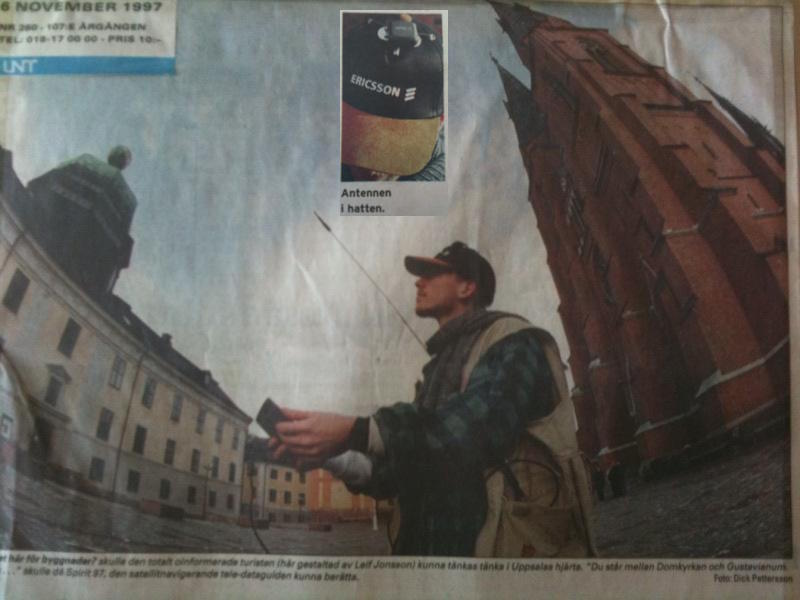
\includegraphics[scale=0.20]{figures/Leif}
	\caption{Me}
	\label{fig:leif}
\end{figure}

\end{columns}
\end{frame}

\begin{frame}
	\frametitle{You}
	\begin{itemize}
		\item Backgound?
		\item Why this course?
		\item Expectations?
	\end{itemize}
\end{frame}

%------------------------------------------------
\section{Course Practicals}
%------------------------------------------------

\begin{frame}
	\frametitle{Course Practicals...}
\end{frame}

\begin{frame}
	\frametitle{Course Practicals...}
	\begin{itemize}
		\item Course code: 732A94
		\item https://www.ida.liu.se/$\sim$732A94/index.en.shtml
		\item https://github.com/MansMeg/AdvRCourse
		\item https://www.rstudio.com/
		\item https://cran.r-project.org/
		\item https://git-scm.com/
	\end{itemize}
\end{frame}


\begin{frame}
	\frametitle{Course litterature...}
\end{frame}

\begin{frame}
	\frametitle{Course litterature...}
	\begin{itemize}
		\item Matloff, N. The art of R programming [online]
		\item Wickham, H. Advanced R [online]
		\item  Wickham, H. R packages [online]
		\item ...and articles.
	\end{itemize}
\end{frame}


\begin{frame}
	\frametitle{Examination}
	Weekly mandatory labs/projects \\
	-- deadline: One week after corresponding lecture \\
	Computer exam
\end{frame}

%------------------------------------------------
\section{Why R?}
%------------------------------------------------

\begin{frame}
	\frametitle{Why R?}
\end{frame}

\begin{frame}
	\frametitle{The One main reason}
	\Huge{\centerline{Choose the right tool for the job!}}
\end{frame}

\begin{frame}
	\frametitle{The One main reason}
	\Huge{\centerline{Choose the right tool for the job!}}
	\Huge{\centerline{ }}
	\large{Your main job will be statistics and data analysis... \\
		 R is the right tool for that job!}
\end{frame}

\begin{frame}
	\frametitle{Pros}
	\begin{itemize}
		\item Popular (among statisticians)
		\item Good graphics support
		\item Open source - all major platforms!
		\item High-level language - focus on data analysis
		\item Strong community - vast amount of packages
		\item Powerful for communicating results
		\item API's to high-performance languages as C/C++ and Java
	\end{itemize}
\end{frame}

\begin{frame}
	\frametitle{Cons}
	\begin{itemize}
		\item ''Ad hoc'', complex, language (Compare Perl, Awk, Sh...)
		\item Can be slooooow
		\item Can be memory inefficient
		\item (Still) Hard'ish to troubleshoot
		\item (Still) Inferior IDE support compared to state of the art
	\end{itemize}
\end{frame}

\begin{frame}
	\frametitle{Pros/Cons}
	\begin{itemize}
		\item Niche language
		\item Specialized syntax
		\item Very permissive
	\end{itemize}
\end{frame}

%------------------------------------------------
\section{Basic R}
%------------------------------------------------

%------------------------------------------------
\subsection{Data structures}
%------------------------------------------------

\begin{frame}
\frametitle{Variable types}
\begin{table}
\begin{tabular}{l l l l l l}
\toprule
&\textbf{Variable type}&\textbf{Short}&\textbf{typeof()}&\textbf{R example}&\\
\midrule
&Boolean & logi & logical & TRUE &\\
&Integer & int & integer & 1L &\\
&Real & num & double & 1.2 &\\
&Complex & cplx & complex & 0+1i &\\
&Character & chr & character & "I \textless3 R" &\\
\bottomrule
\end{tabular}
\end{table}
\end{frame}


\begin{frame}
	\frametitle{Variable types}
	\begin{table}
		\begin{tabular}{c l l l l c}
			\toprule
			&\textbf{Variable type}&\textbf{Short}&\textbf{typeof()}&\textbf{R 
			example}&\\
			\midrule
			$\Downarrow$ & Boolean & logi & logical & TRUE & $\Downarrow$\\
			 & Integer & int & integer & 1L &\\
			Coersion& Real & num & double & 1.2 & Coersion\\
			&Complex & cplx & complex & 0+1i &\\
			$\Downarrow$&Character & chr & character & "I \textless3 R" & 
			$\Downarrow$\\
			\bottomrule
		\end{tabular}
	\end{table}
\end{frame}

\begin{frame}
	\frametitle{Data structures}
	\begin{table}
		\begin{tabular}{l l l}
			\toprule
			\textbf{Dimension}&\textbf{Homogeneous data}&\textbf{Heterogeneous 
			data}\\
			\midrule
			1 & vector & list \\
			2 & matrix & data.frame \\
			n & array &  \\
			\bottomrule
		\end{tabular}
	\end{table}
	
		\begin{itemize}
			\item Constructors: vector() list() ...
			\item Name dimensions: dimnames()
		\end{itemize}
\end{frame}


\begin{frame}
	\frametitle{Arithmetics}
	\begin{itemize}
		\item Vectorized operations (element wise)
		\item Recycling
		\item Statistical functions
	\end{itemize}
	
	See reference card...
\end{frame}

%------------------------------------------------
\subsection{Logic and sets}
%------------------------------------------------

\begin{frame}
	\frametitle{Logic operators}
	\begin{table}
		\begin{tabular}{l l l l l l}
			\toprule
			In symbols & A & B & $\neg$A & A$\land$B & A$\lor$B\\
			In R & $A$ & $B$ & $!A$ & A\&B & $A \vert B$ \\
			& TRUE & FALSE & ? & ? & ? \\
			& TRUE & TRUE & ? & ? & ? \\
			& FALSE & FALSE & ? & ? & ? \\
			& FALSE & TRUE & ? & ? & ? \\
			\bottomrule
		\end{tabular}
	\end{table}
\end{frame}

\begin{frame}
	\frametitle{Logic operators}
	\begin{table}
		\begin{tabular}{l l l l l l}
			\toprule
			In symbols & A & B & $\neg$A & A$\land$B & A$\lor$B\\
			In R & $A$ & $B$ & $!A$ & A\&B & $A \vert B$ \\
			& TRUE & FALSE & FALSE & ? & ? \\
			& TRUE & TRUE & ? & ? & ? \\
			& FALSE & FALSE & ? & ? & ? \\
			& FALSE & TRUE & ? & ? & ? \\
			\bottomrule
		\end{tabular}
	\end{table}
\end{frame}

\begin{frame}
	\frametitle{Logic operators}
	\begin{table}
		\begin{tabular}{l l l l l l}
			\toprule
			In symbols & A & B & $\neg$A & A$\land$B & A$\lor$B\\
			In R & $A$ & $B$ & $!A$ & A\&B & $A \vert B$ \\
			& TRUE & FALSE & FALSE & FALSE & ? \\
			& TRUE & TRUE & ? & ? & ? \\
			& FALSE & FALSE & ? & ? & ? \\
			& FALSE & TRUE & ? & ? & ? \\
			\bottomrule
		\end{tabular}
	\end{table}
\end{frame}

\begin{frame}
	\frametitle{Logic operators}
	\begin{table}
		\begin{tabular}{l l l l l l}
			\toprule
			In symbols & A & B & $\neg$A & A$\land$B & A$\lor$B\\
			In R & $A$ & $B$ & $!A$ & A\&B & $A \vert B$ \\
			& TRUE & FALSE & FALSE & FALSE & TRUE \\
			& TRUE & TRUE & ? & ? & ? \\
			& FALSE & FALSE & ? & ? & ? \\
			& FALSE & TRUE & ? & ? & ? \\
			\bottomrule
		\end{tabular}
	\end{table}
\end{frame}

\begin{frame}
	\frametitle{Logic operators}
	\begin{table}
		\begin{tabular}{l l l l l l}
			\toprule
			In symbols & A & B & $\neg$A & A$\land$B & A$\lor$B\\
			In R & $A$ & $B$ & $!A$ & A\&B & $A \vert B$ \\
			& TRUE & FALSE & FALSE & FALSE & TRUE \\
			& TRUE & TRUE & FALSE & TRUE & TRUE \\
			& FALSE & FALSE & TRUE & FALSE & FALSE \\
			& FALSE & TRUE & TRUE & FALSE & TRUE \\
			\bottomrule
		\end{tabular}
	\end{table}
\end{frame}

\begin{frame}
	\frametitle{Logic operators}
	\begin{table}
		\begin{tabular}{l l l l}
			\toprule
			In symbols & $\land_{i=1}^{N}a_i$ & $\lor_{i=1}^{N}a_i$ & $\{j : 
			a_j==TRUE\}$\\
			In R & $all(A)$ & $any(A)$ & $which(A)$ \\
			\bottomrule
		\end{tabular}
	\end{table}
\end{frame}


\begin{frame}
	\frametitle{Relational operators}
	\begin{table}
		\begin{tabular}{l l l l l l}
			\toprule
			In symbols & $a \textless b$ & $a \leq  b$ & $a \neq  b$ & $a =  
			b$ & $a \in b$ \\
			In R & $a < b$ & $a <= b$ & $a != b$ & a == b & a \%in\% b \\
			\bottomrule
		\end{tabular}
	\end{table}
\end{frame}

%------------------------------------------------
\subsection{Subsetting/filtering}
%------------------------------------------------

\defverbatim[colored]\lstI{
	\begin{lstlisting}[language=R,basicstyle=\ttfamily,keywordstyle=\color{red},
	 basicstyle=\small]
	vect <- c(6,7,8,9)
	> vect[vect>7]
	[1] 8 9
	> vect[1:2]
	[1] 6 7
	> vect[c(1,2)]
	[1] 6 7
	> vect[c(-1,-2)]
	[1] 8 9
	\end{lstlisting}
}

\begin{frame}
	\frametitle{Vectors}
	\begin{itemize}
		\item Use []
		\item index by:
			\begin{itemize}
				\item positive integers: include element(s)
				\item negative integers: exclude element(s)
				\item logical: include TRUEs
			\end{itemize}
	\end{itemize}
	\lstI
\end{frame}

\defverbatim[colored]\lstII{
	\begin{lstlisting}[language=R,basicstyle=\ttfamily,keywordstyle=\color{red},
	basicstyle=\small]
	> mat <- matrix(c(1,2,3,4,5,6),nrow=2)
	> mat
	      [,1] [,2] [,3]
	[1,]    1    3    5
	[2,]    2    4    6
	> mat[c(1,2),c(1,2)]
	      [,1] [,2]
	[1,]    1    3
	[2,]    2    4
	> mat[c(1,2),]
	      [,1] [,2] [,3]
	[1,]    1    3    5
	[2,]    2    4    6
	> mat[mat>4]
	[1] 5 6
	\end{lstlisting}
}

\begin{frame}
	\frametitle{Matrices}
	\begin{itemize}
		\item Use [,]
		\item Two dimensions
		\item Index as vectors
		\item Can reduce (drop class) to vector
	\end{itemize}
\end{frame}

\begin{frame}
	\frametitle{Matrices}
	\lstII
\end{frame}

\defverbatim[colored]\lstIII{
	\begin{lstlisting}[language=R,basicstyle=\ttfamily,keywordstyle=\color{red},
	basicstyle=\small]
> lst <- list(a=47,b=11)
> lst[1]
$a
[1] 47

> lst[[1]]
[1] 47
> lst$b
[1] 11
\end{lstlisting}
}

\begin{frame}
	\frametitle{Lists}
	\begin{itemize}
		\item Use [] to access list elements
		\item Use [[]] to access list content
		\item Index as vectors
		\item Use \$ to access list element by name
		\item Not like typical lists in other programming languages
	\end{itemize}
\end{frame}

\begin{frame}
	\frametitle{Lists}
	\lstIII
\end{frame}

\begin{frame}
	\frametitle{Data frames}
	\begin{itemize}
		\item Very powerful data structure
		\item Can roughly think about it as the R representation of a CSV file
		\item Can be loaded from a CSV file
		\item Can be accessed both as a matrix and a list
	\end{itemize}
\end{frame}


\begin{frame}
	\frametitle{Assigning subsets}
	\begin{itemize}
		\item Change values in data structures
		\item Works for all above mentioned data types 
	\end{itemize}
\end{frame}

\defverbatim[colored]\lstIIII{
	\begin{lstlisting}[language=R,basicstyle=\ttfamily,keywordstyle=\color{red},
	basicstyle=\small]
> mat
      [,1] [,2] [,3]
[1,]    1    3    5
[2,]    2    4    6
> mat[mat>4] = 75
> mat
      [,1] [,2] [,3]
[1,]    1    3   75
[2,]    2    4   75
\end{lstlisting}
}

\begin{frame}
	\frametitle{Assigning subsets}
	\lstIIII
\end{frame}

%------------------------------------------------
\subsection{Functions}
%------------------------------------------------

\defverbatim[colored]\lstV{
	\begin{lstlisting}[language=R,basicstyle=\ttfamily,keywordstyle=\color{black},
	basicstyle=\small]
	my_function_name <- function(x, y){
		z <- x^2 + y^2
		return(z)
	}
	\end{lstlisting}
}

\begin{frame}
	\frametitle{Functions}
	\lstV
	Unlike in many languages, \texttt{return} in R is a \textbf{function}.
	In other languages, \texttt{return} is usually a \textbf{reserved word} 
	(like \texttt{if}). This means you must use \texttt{return} as a function 
	call with parenthesis. By default R returns the last computed value of the 
	function, so return is not strictly necessary in simple cases.
\end{frame}

%------------------------------------------------

\begin{frame}
\Huge{\centerline{The End... for today.}}
\Huge{\centerline{Questions?}}
\Huge{\centerline{See you next time!}}
\end{frame}

%----------------------------------------------------------------------------------------

\end{document} 